\subsection{Comparación de algoritmos}

En esta sección, comparamos varios algoritmos con respecto a nuestras métricas de interés: Accuracy, Precision, Recall y F1 Score (R2). Los algoritmos considerados se dividen en:

\subsubsection*{Clasificación:}

\begin{itemize}
    \item DecisionTreeClassifier
    \item LogisticRegression
    \item RandomForestClassifier
    \item XGBClassifier
\end{itemize}

Para estos modelos, se utilizará la variable objetivo \say{aprobado}, la técnica \say{Stratified K-Fold Cross-Validation}, ajustaremos el mejor modelo en los datos de entrenamiento y realizaremos predicciones utilizando el mejor modelo.

La mejor configuración para los modelos de clasificación se muestra en la Figura \ref{fig:config_clasifiacion}:

\begin{figure}[H]
    \centering
    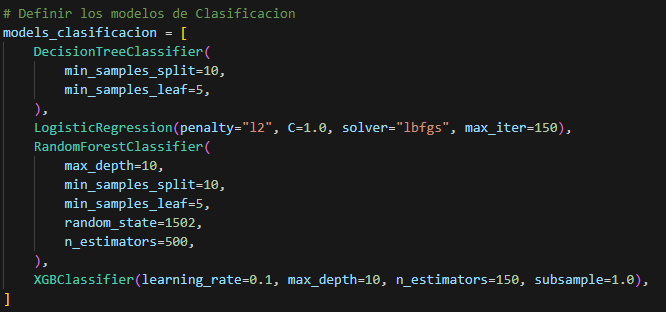
\includegraphics[width=6.0611in,height=2.6861in]{img/compara_algoritmos/configModelsClasificacion.png}
    \caption{Configuración de los modelos de clasificación}
    \label{fig:config_clasifiacion}
\end{figure}

Los resultados obtenidos para el conjunto de entrenamiento se presentan en la Figura \ref{fig:metricas_clasificacion}:

\begin{figure}[H]
    \centering
    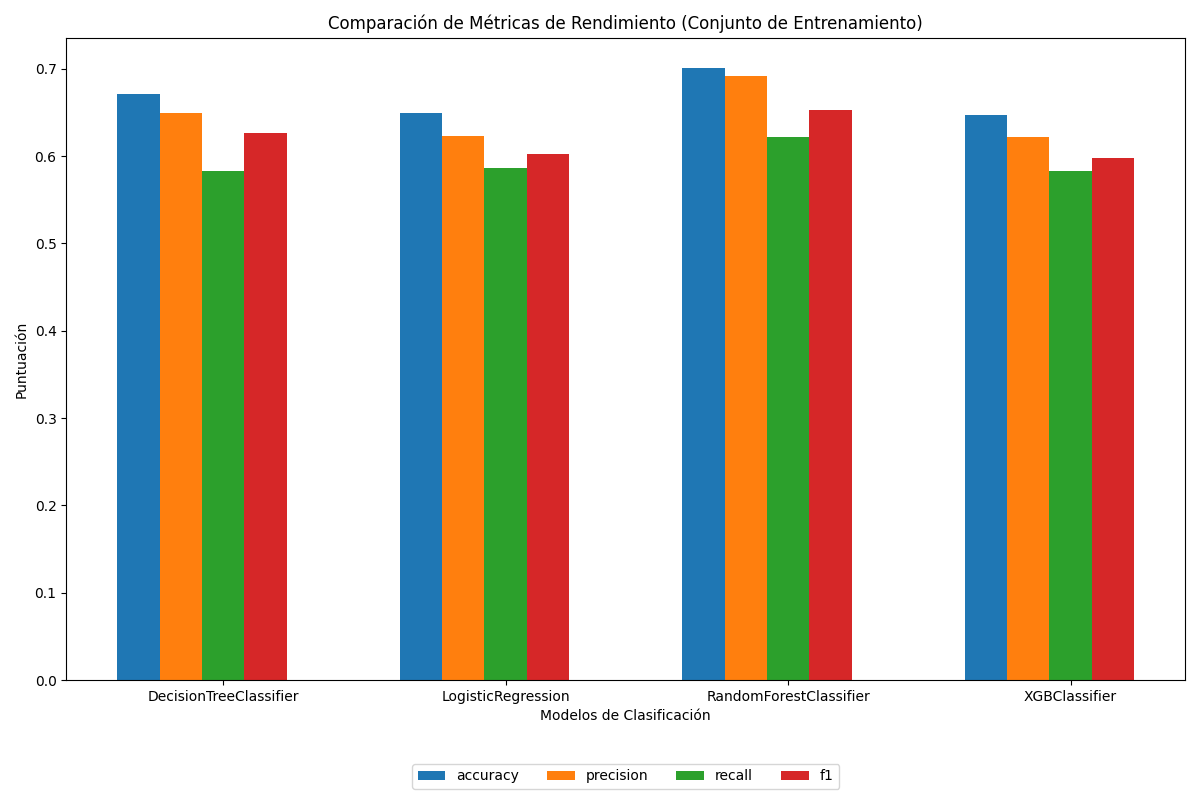
\includegraphics[width=7.06111in,height=4.68611in]{img/compara_algoritmos/metricasEntreModelosClasificacion.png}
    \caption{Métricas entre modelos de clasificación conjunto de entrenamiento}
    \label{fig:metricas_clasificacion}
\end{figure}

En la figura se observa que el modelo RandomForestClassifier es el mejor modelo, con un F1 Score del 62.53\%, un recall del 58.90\%, una precisión del 66.54\% y una exactitud del 67.61\%, en comparación con los otros modelos evaluados.

Los resultados sobre el conjunto de prueba se presentan en la figura \ref{fig:metricas_clasificacion_bestModel}

\begin{figure}[H]
    \centering
    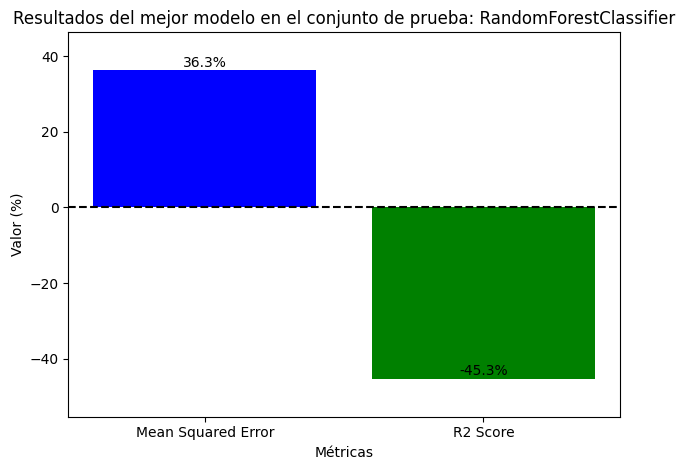
\includegraphics[width=7.06111in,height=4.68611in]{img/compara_algoritmos/metricasBestModelRandomForesClassifier.png}
    \caption{Métricas best model de clasificación}
    \label{fig:metricas_clasificacion_bestModel}
\end{figure}

con resultados en Mean Squared Error: 36.3 \%  y R2 Score: -45.3\%

En conclucion y en base en los resultados obtenidos, se puede concluir que el modelo RandomForestClassifier es el más adecuado para problemas de clasificación.

\begin{itemize}
    \item El mejor modelo en la validación fue: RandomForestClassifier 62.53\%
\end{itemize}

Resultados del mejor modelo en el conjunto de prueba:

\begin{itemize}
    \item Mean Squared Error: 36.3\%
    \item R2 Score: -45.3\%
\end{itemize}

\subsubsection*{Regresión:}

\begin{itemize}
    \item LinearRegression
    \item DecisionTreeRegressor
    \item KNeighborsRegressor
\end{itemize}

Para estos modelos, se utilizará la variable objetivo \say{sol1}, la técnica \say{K-Fold Cross-Validation}, ajustaremos el mejor modelo en los datos de entrenamiento y realizaremos predicciones utilizando el mejor modelo.

La mejor configuración para los modelos de regresión se muestra en la Figura \ref{fig:config_regresion}:

\begin{figure}[H]
    \centering
    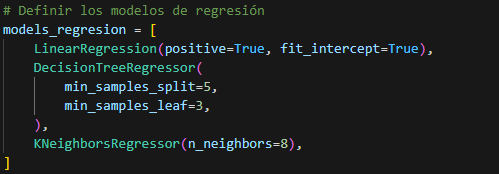
\includegraphics[width=5.06111in,height=1.68611in]{img/compara_algoritmos/configModelsRegresion.png}
    \caption{Configuración de los modelos de regresión}
    \label{fig:config_regresion}
\end{figure}

Los resultados obtenidos se presentan en la Figura \ref{fig:metricas_regresion}:

\begin{figure}[H]
    \centering
    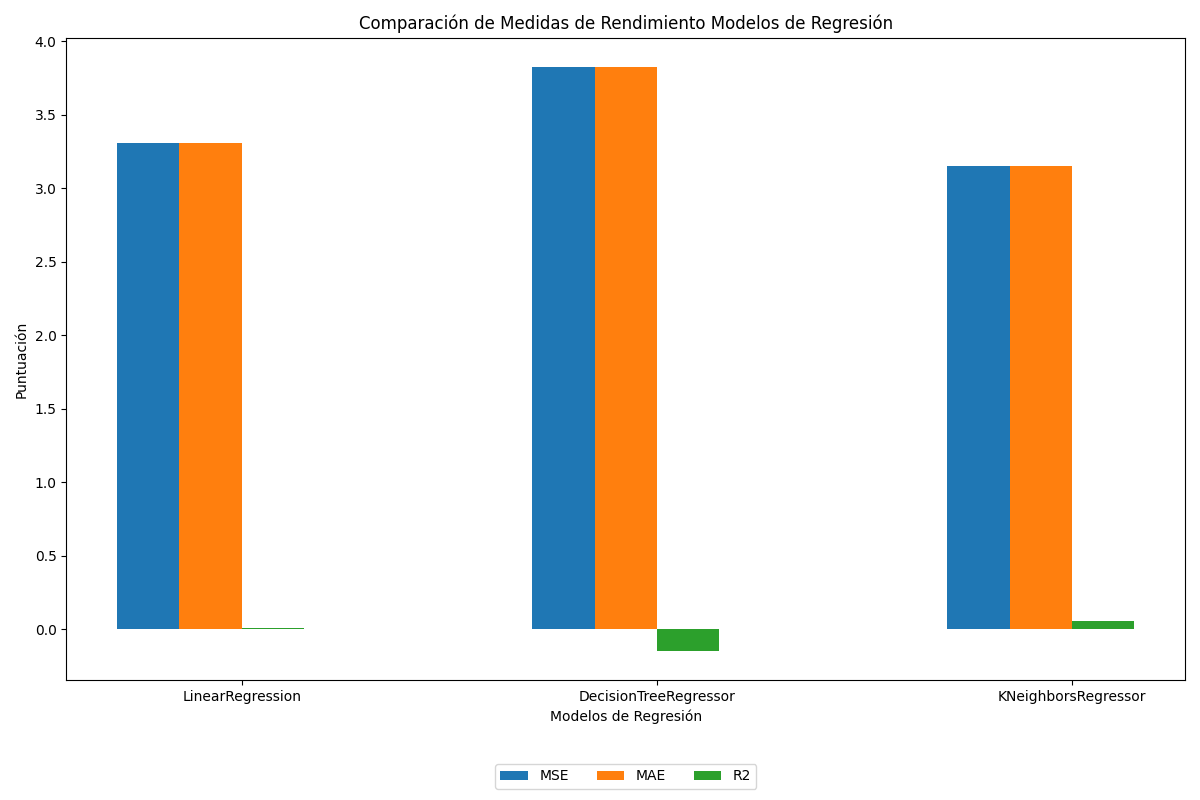
\includegraphics[width=7.06111in,height=4.68611in]{img/compara_algoritmos/metricasEntreModelosRegresion.png}
    \caption{Métricas entre modelos de regresión conjunto de entrenamiento}
    \label{fig:metricas_regresion}
\end{figure}

Se observa que el modelo LinearRegression en su conjunto de entrenamiento presenta el comportamiento mas normal utilizando la validacion k-fold cross-validation para variables cuantitativas.

Los resultados sobre el conjunto de prueba se presentan en la figura \ref{fig:metricas_regresion_bestModel}

\begin{figure}[H]
    \centering
    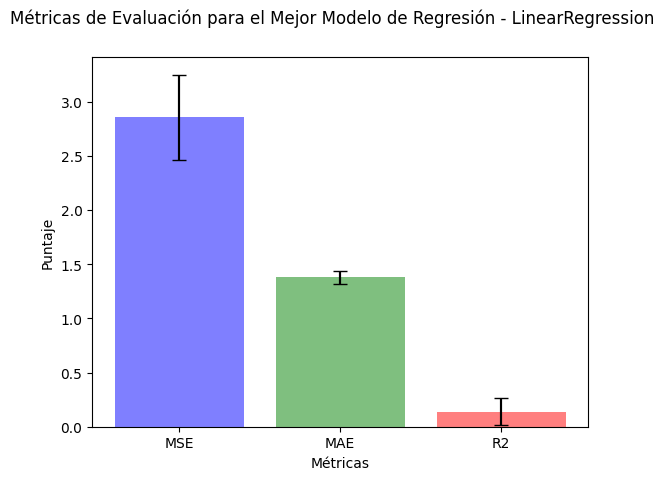
\includegraphics[width=7.06111in,height=4.68611in]{img/compara_algoritmos/metricasBestModelLinearRegression.png}
    \caption{Métricas Best Model}
    \label{fig:metricas_regresion_bestModel}
\end{figure}

Se observa que el modelo LinearRegression es el mejor modelo de regresión, con un MSE del 3.6\% y un MAE del 1.6\%, valores inferiores a los de los otros modelos evaluados. Además, el modelo LinearRegression presenta un R2 más cercano a 1, con un aumento del 0.1\% en comparación con los demás modelos.

En base en los resultados obtenidos, se puede concluir que el modelo LinearRegression es el más adecuado para problemas de regresion con variable cuantitativas.

\begin{itemize}
    \item El mejor modelo en la validación fue: LinearRegression 14.1\%
\end{itemize}

Resultados del mejor modelo en el conjunto de prueba:

\begin{itemize}
    \item MSE: 3.6.\%
    \item MAE: 1.6\%
    \item R2: 0.1\%
\end{itemize}

En conclusión, se realizó una comparación exhaustiva de diferentes algoritmos de modelos predictivos para determinar cuál es el más adecuado en términos de origen de datos. Después de analizar y comparar varios algoritmos, se llegó a la conclusión de que el modelo RandomForestClassifier se destaca como el enfoque más efectivo para el origen de datos en cuestión, mientras que el modelo LinearRegression es el más adecuado para análisis de regresión.